\chapter{Systematic uncertainties}
\label{chap:systematics}
In this section, all systematic uncertainties considered in the analysis are described. 
Systematic uncertainty is treated as nuisance parameter in the statistical analysis, and is estimated with respect to the final dicriminants.
Each systematic uncertainty is considered to be the combination of two elements, normalization uncertainty and the shape uncertainty. 
Normalization uncerintainty is the uncertainty of the yields compared to the nominal yields in each region, while shape uncertainty is the variation of the shape of the discriminant, when the yields are normalized.
The source of the uncertainties are classified into two categories; the experimental uncertainties, mainly come from the reconstruction and calibration of the physics objects, and the theory uncertainties, come from the modeling or the theoretical calculation of the signal and background MC samples.
Each uncertainty in two categories considered in the analysis is discussed in the following sections.

\section{Experimental uncertainties}
\label{sec:ExperimUnc}
\noindent\textbf{\sf{Luminosity}}\\
The uncertainty on the integrated luminosity, obtained using the LUCID-2 detector for the primary luminosity measurements for the 2015+2016 dataset is 2.1\%, and 2.4\% for the 2017 dataset. The uncertainty for the 2018 data alone is 2.0\%, and the uncertainty for the combined run-2 dataset (2015-2018) is 1.7\% The combined uncertainty is applied to all MC samples. \cite{AtlasLumiRun2}. \\ 
\\
\noindent\textbf{\sf{Pileup reweighting}}\\
The MC events are weighted in order to match $\mu$ of the MC, the average number of interactions per bunch crossing, to that of data. 
The pileup reweighting uncertainty is estimated by changing its scaling. \\
\\
\noindent\textbf{\sf{Leptons}}\\
The uncertainties related to the lepton triggers are negligible, since their efficiencies are almost 100~\%.
The uncertainties from the reconstruction and identification, and the calibration of the energy scale and resolution described in chapter~\ref{chap:reconstruction} is considered. The variations are order of 1~\%. \\
\\
\noindent\textbf{\sf{Small-R jets}}\\
Uncertainties on the jet energy scale (JES)  and the jet energy resolution (JER) are considered.
The JES and JER are measured in situ by calculating the response between MC and data, as detailed in chapter~\ref{chap:reconstruction}. 
The uncertainties on the efficiency of the pile-up jets and the forward vertex tagger, and the tracking reconstruction uncertainties are also considered, as well as b-tagging tool uncertainties.
The impacts from these uncertainties are expected to be low, as they are less than 5~\% in the high RNN bins of the signal regions. 
%Flavour response/composition uncertainties 
\\
\\
\noindent\textbf{\sf{Large-R jets}}\\
JES and JER uncertainties are also considered with large-R jet.  
Uncertainty related to the boson tagger efficiency scale factors (SFs) \cite{ATL-PHYS-PUB-2015-053} are considered. 
The scale factors that correct the tagger efficiency in simulation to match that in data are derived from data using t$\bar{\mathrm{t}}$ events for signal-like labelled jets, while extracted from $\gamma$+jet and multijet events for background jets.
There are several sources of uncertainties, including the theoretical uncertainty in the MC samples used for deriving the SFs, as well as, reconstruction of calibration of the physics objects. 
This uncertainty is designed to change the ratio of the normalization between CR and the SR.

%\subsection{Quark/Gluon jets uncertainties}
%The Flavour response and the Flavour composition uncertainties are derived specifically to this analysis.
%These two uncertainties explain the different jets response to quark and gluon-initiated jets. The flavour response uncertainty is derived by using the dijet events used the alternative samples, which are Phythia~8 and Herwig~$\plus\plus$. The flavour composition uncertainty is usually derived by assuming 50\% quarks and 50\% gluons and takes conservative uncertainty of 100\%, though it is too conservative uncertainties and can limit the sensitivities in topology of this analysis, where quark enriched regions are expected. In order to reduce these uncertainties, the gluon fraction is studied and these uncertainties are re-derived using specific gluon fraction.

%how to derive this 
%The gluon fraction in each of the analysis regions and different samples is estimated as a function of the $p_T$ and $\eta$ for small-R jets. Truth parton label information is used to estimating the number of quarks and gluons. All jets except the b-quark-initiated jets are into account.
%The gluon fraction for a given bin of the 2D histograms of $p_T$ and $eta$ after summing up all the region is taken as the nominal gluon fraction. As to describe the uncertainty on the gluon fraction, it is given by:
%\begin{equation}
%\sigma_{gfrac}=\sqrt{\sigma_{\text {region }}^{2}+\sigma_{g e n}^{2}}
%\end{equation}
%where $\sigma_{region}$ is the maximum difference in nominal gluon fraction and the one analysis region, and $\sigma_{gen}$ is the generator uncertainty derived using alternative Pythia 8 and Herwig MC samples. For Signal samples there is no alternative MC sample available, only region uncertainty is considered.

\section{Theory uncertainties}
\label{sec:TheoryUnc}
%The systematic uncertainties related to the determination or the calculation of the MC of the theoretical modeling of the simulated signal and background processes are considered.
For the main sources of the background samples, only shapes of these theoretical uncertainties are considered in the final fitting. 
The normalization is not included in the fitting, since it is determined by the free normalization factor in the fit from the data in CRs.

\subsection{Reweighting uncertainties}
As described in chapter~\ref{chap:modeling}, the $m^{tag}_{jj}$ reweighting is applied to the V+jet background, and the distribution is corrected. 
The dedicated uncertainty is assigned conservatively, considering a 100~\% uncertainty on the linear fit parameter; the distribution without the correction is used as a pre-fit $-1~\sigma$ variation; and the uncertainty is symmetrized to define $+1~\sigma$ variation. 
The pre-fit variation of the Z+jets sample in the 2-lepton channel is shown in figure~\ref{fig:mjjreweighting}.
The reweighting uncertainty is estimated in the CRs and propagated to the SRs with an event-by-event weight. 
To cover the possible remaining mis-modeling with the RNN score considering that the modeling is different between $m^{tag}_{jj}$ and the RNN score, this uncertainty is designed to be large and enough conservatively.
\begin{figure}[H]
\begin{center}
 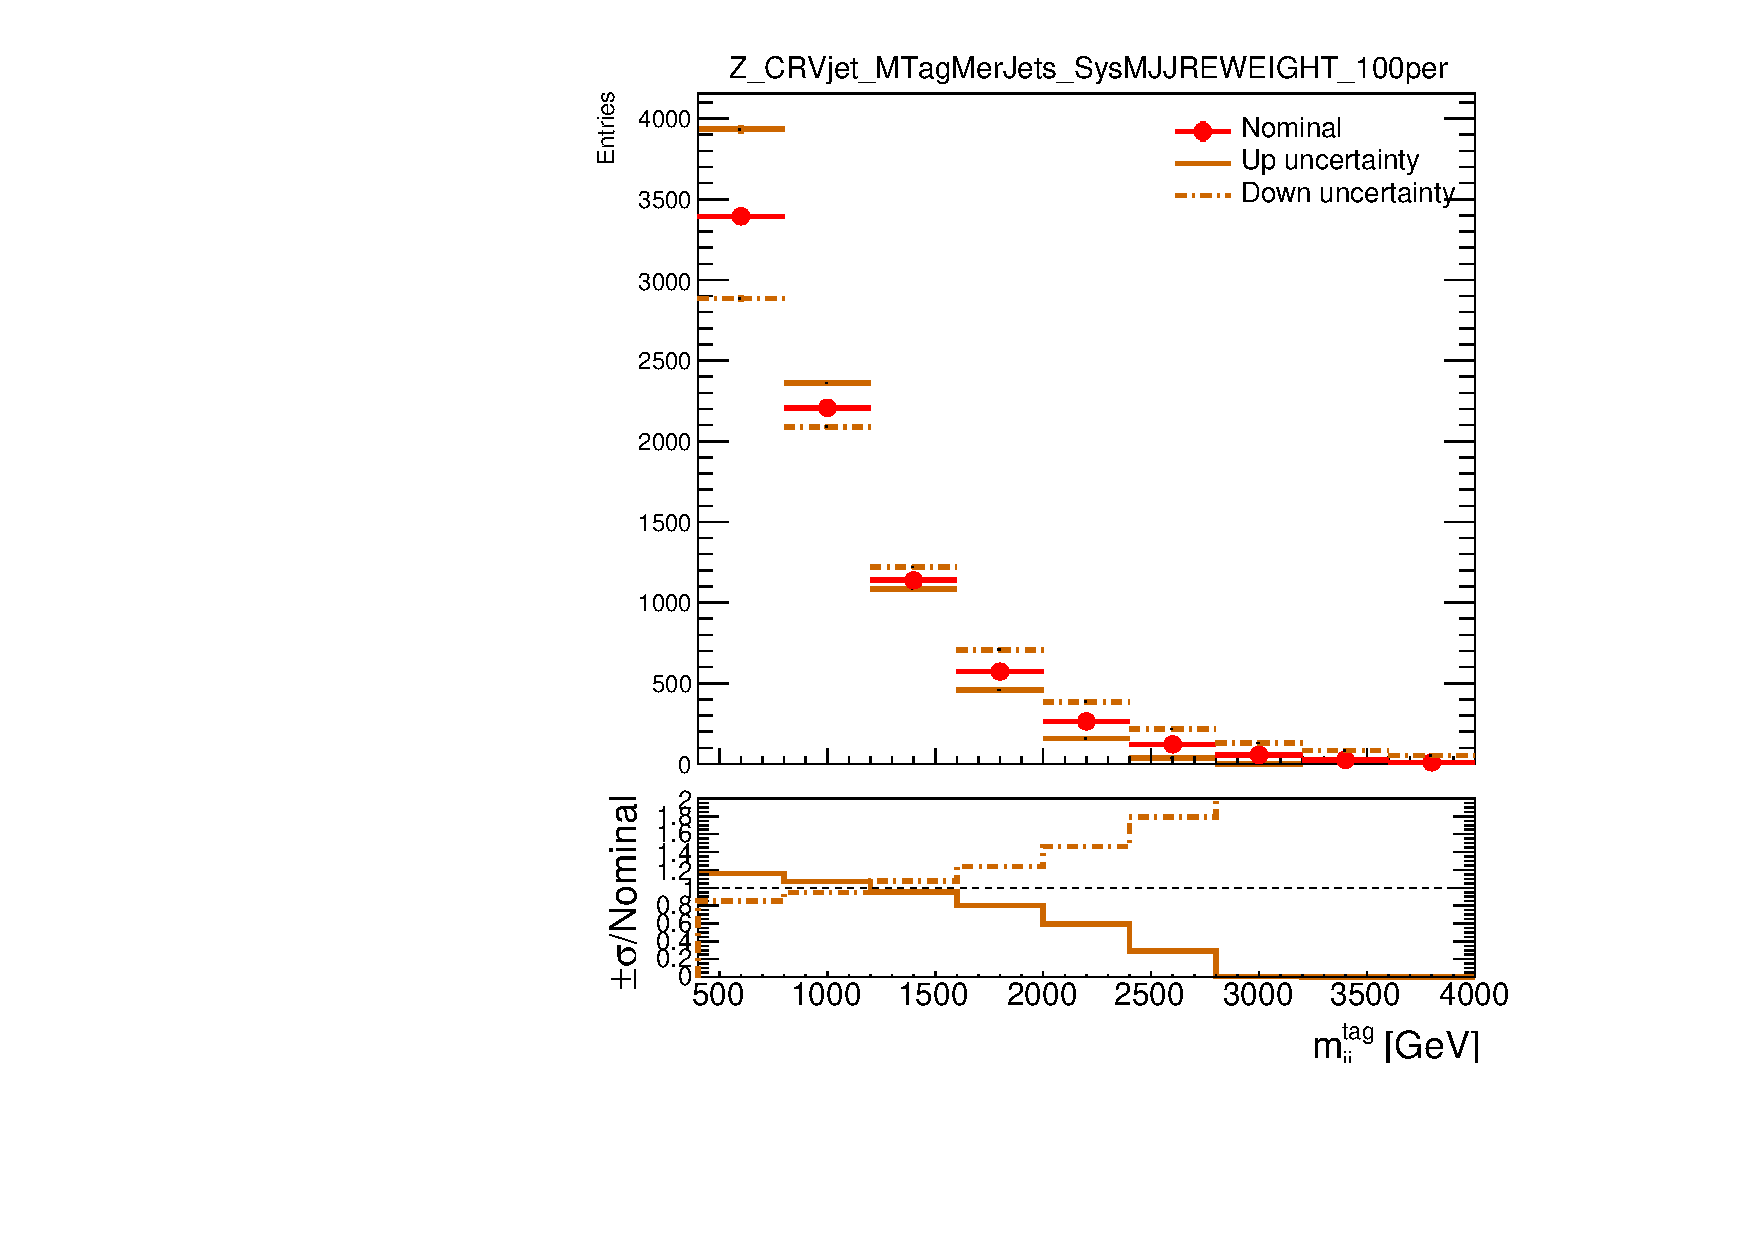
\includegraphics[width=0.32\textwidth,keepaspectratio]{figures/syst/Z_0ptag1pfat0pjet_0ptv_CRVjet_MTagMerJets_SysMJJREWEIGHT_100per.pdf}
 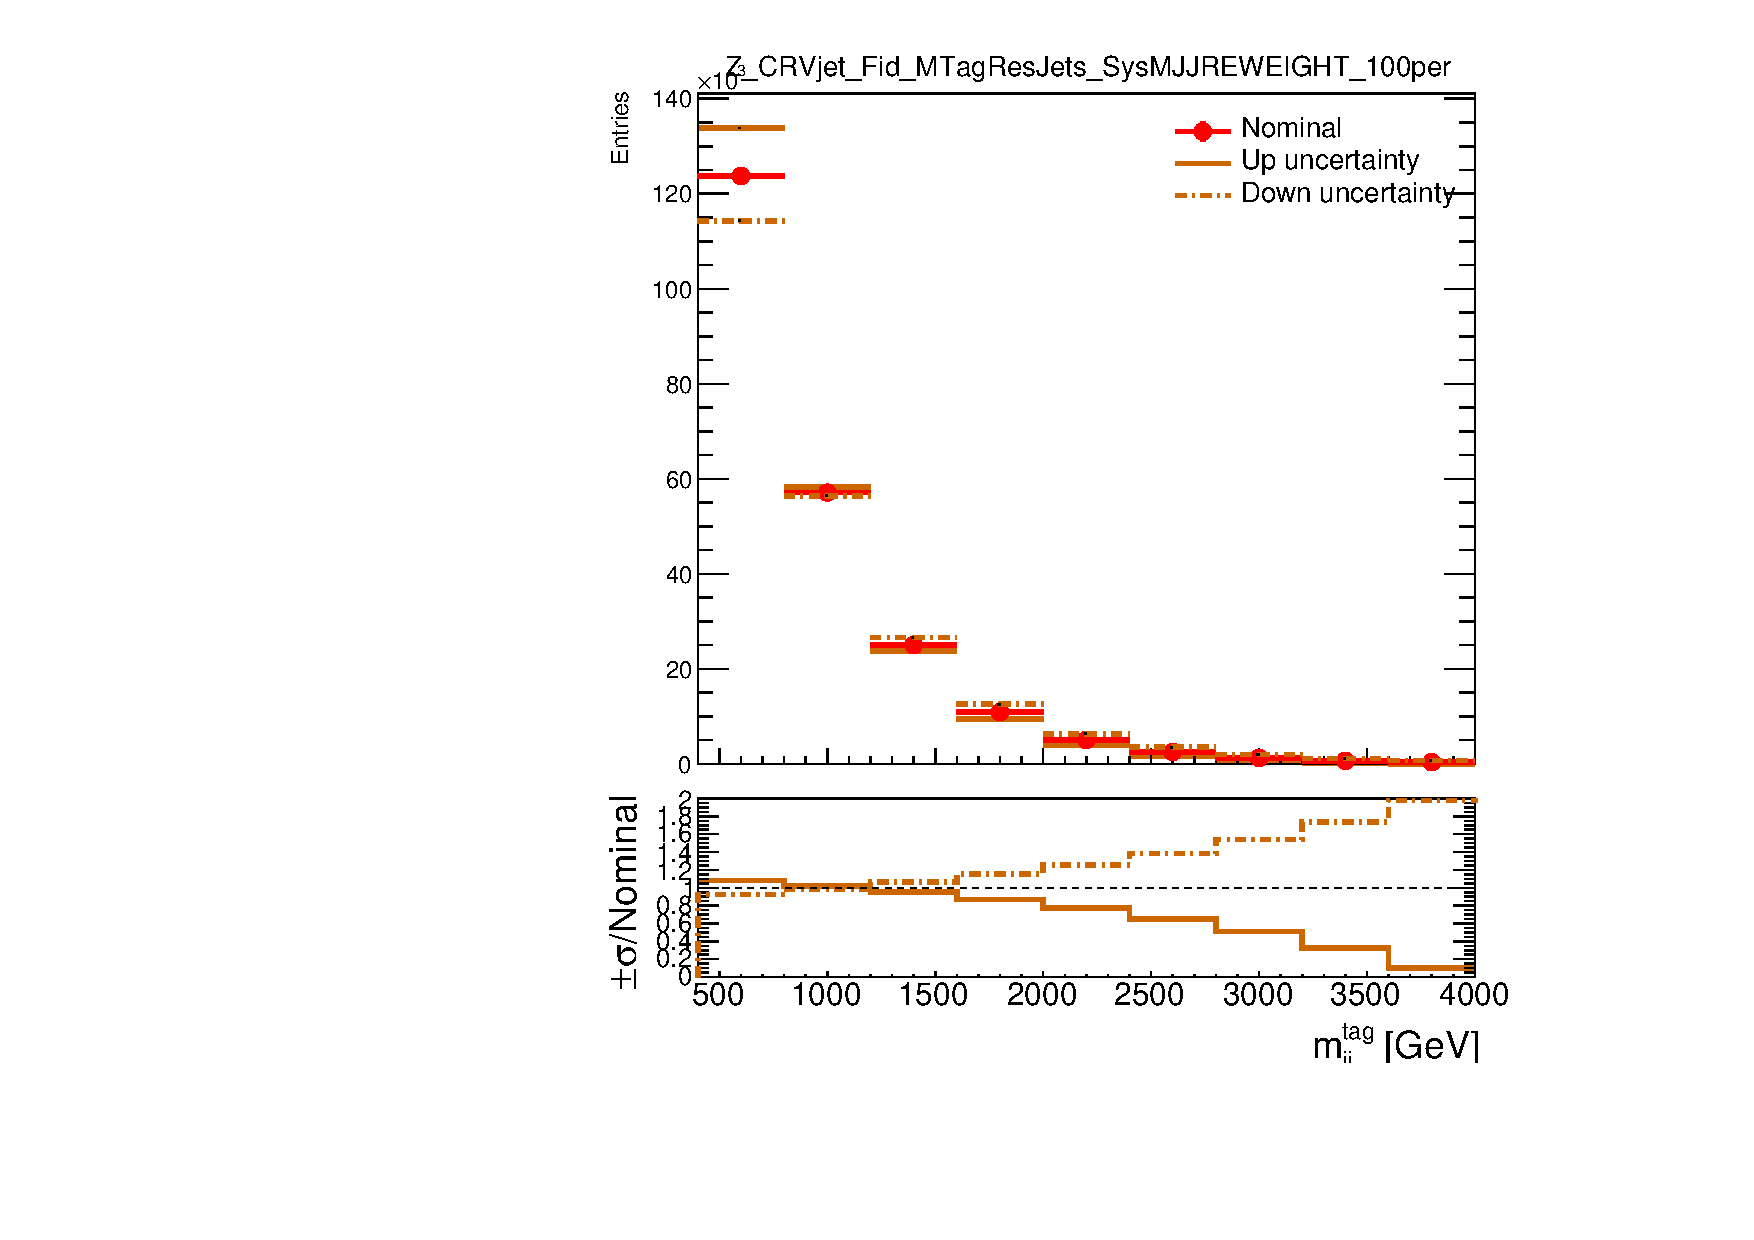
\includegraphics[width=0.32\textwidth,keepaspectratio]{figures/syst/Z_0ptag2pjet_0ptv_CRVjet_Fid_MTagResJets_SysMJJREWEIGHT_100per.pdf}
 \\
 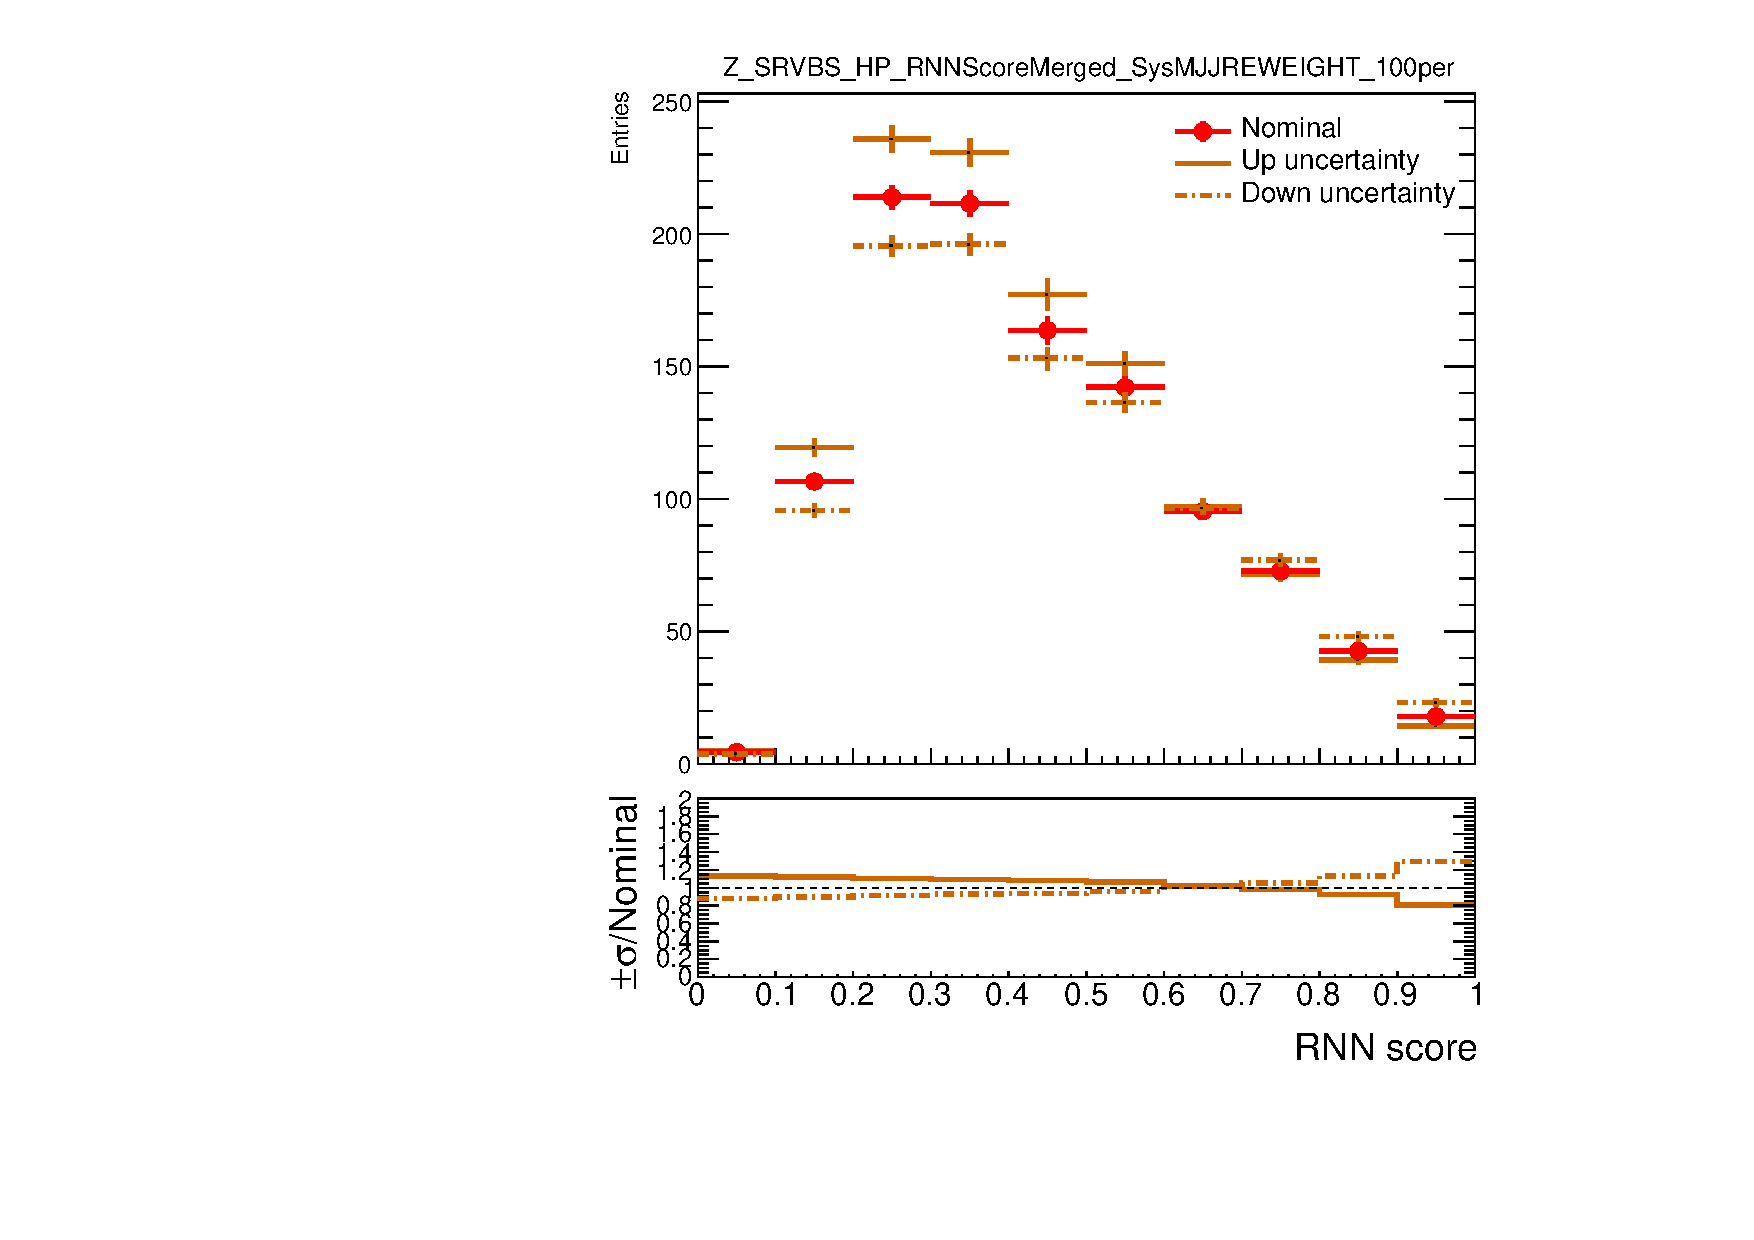
\includegraphics[width=0.32\textwidth,keepaspectratio]{figures/syst/Z_0ptag1pfat0pjet_0ptv_SRVBS_HP_RNNScoreMerged_SysMJJREWEIGHT_100per.pdf}
 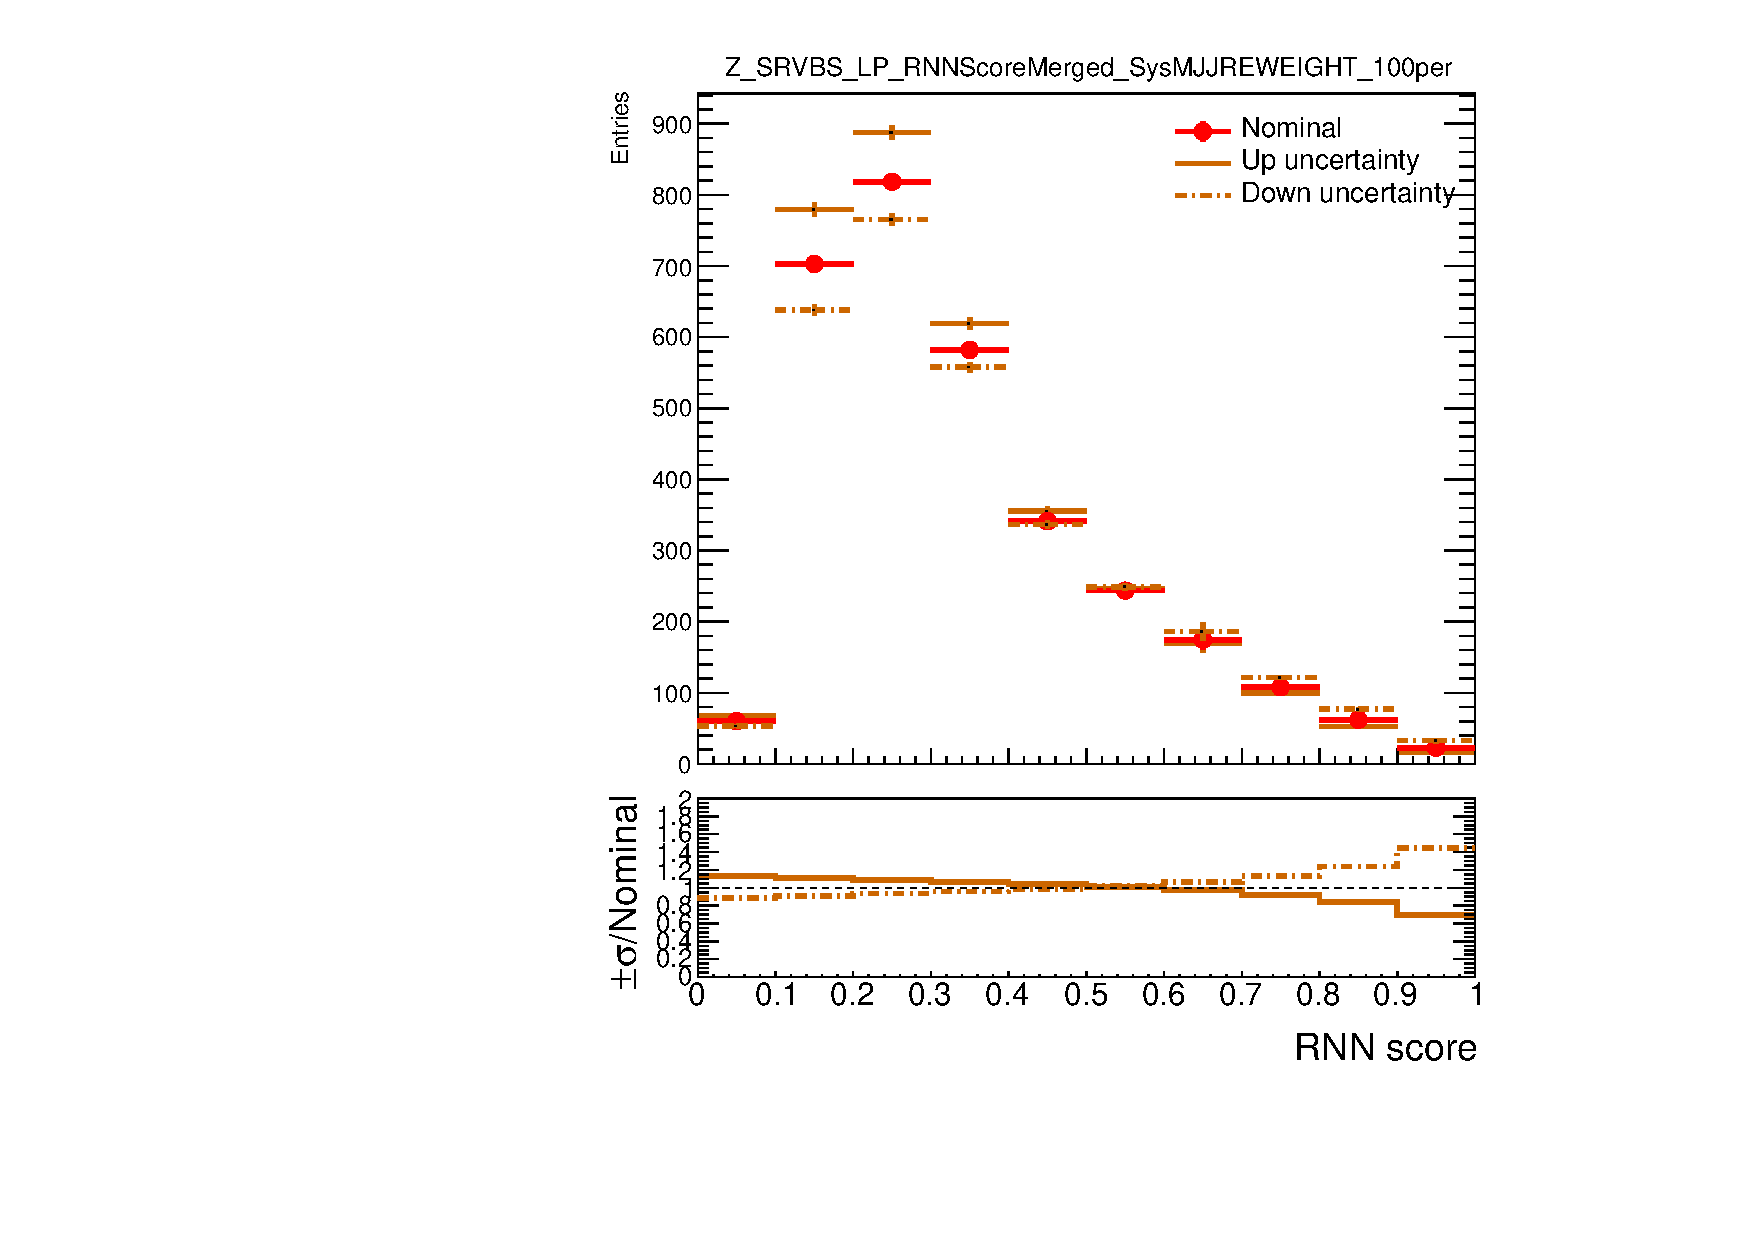
\includegraphics[width=0.32\textwidth,keepaspectratio]{figures/syst/Z_0ptag1pfat0pjet_0ptv_SRVBS_LP_RNNScoreMerged_SysMJJREWEIGHT_100per.pdf}
 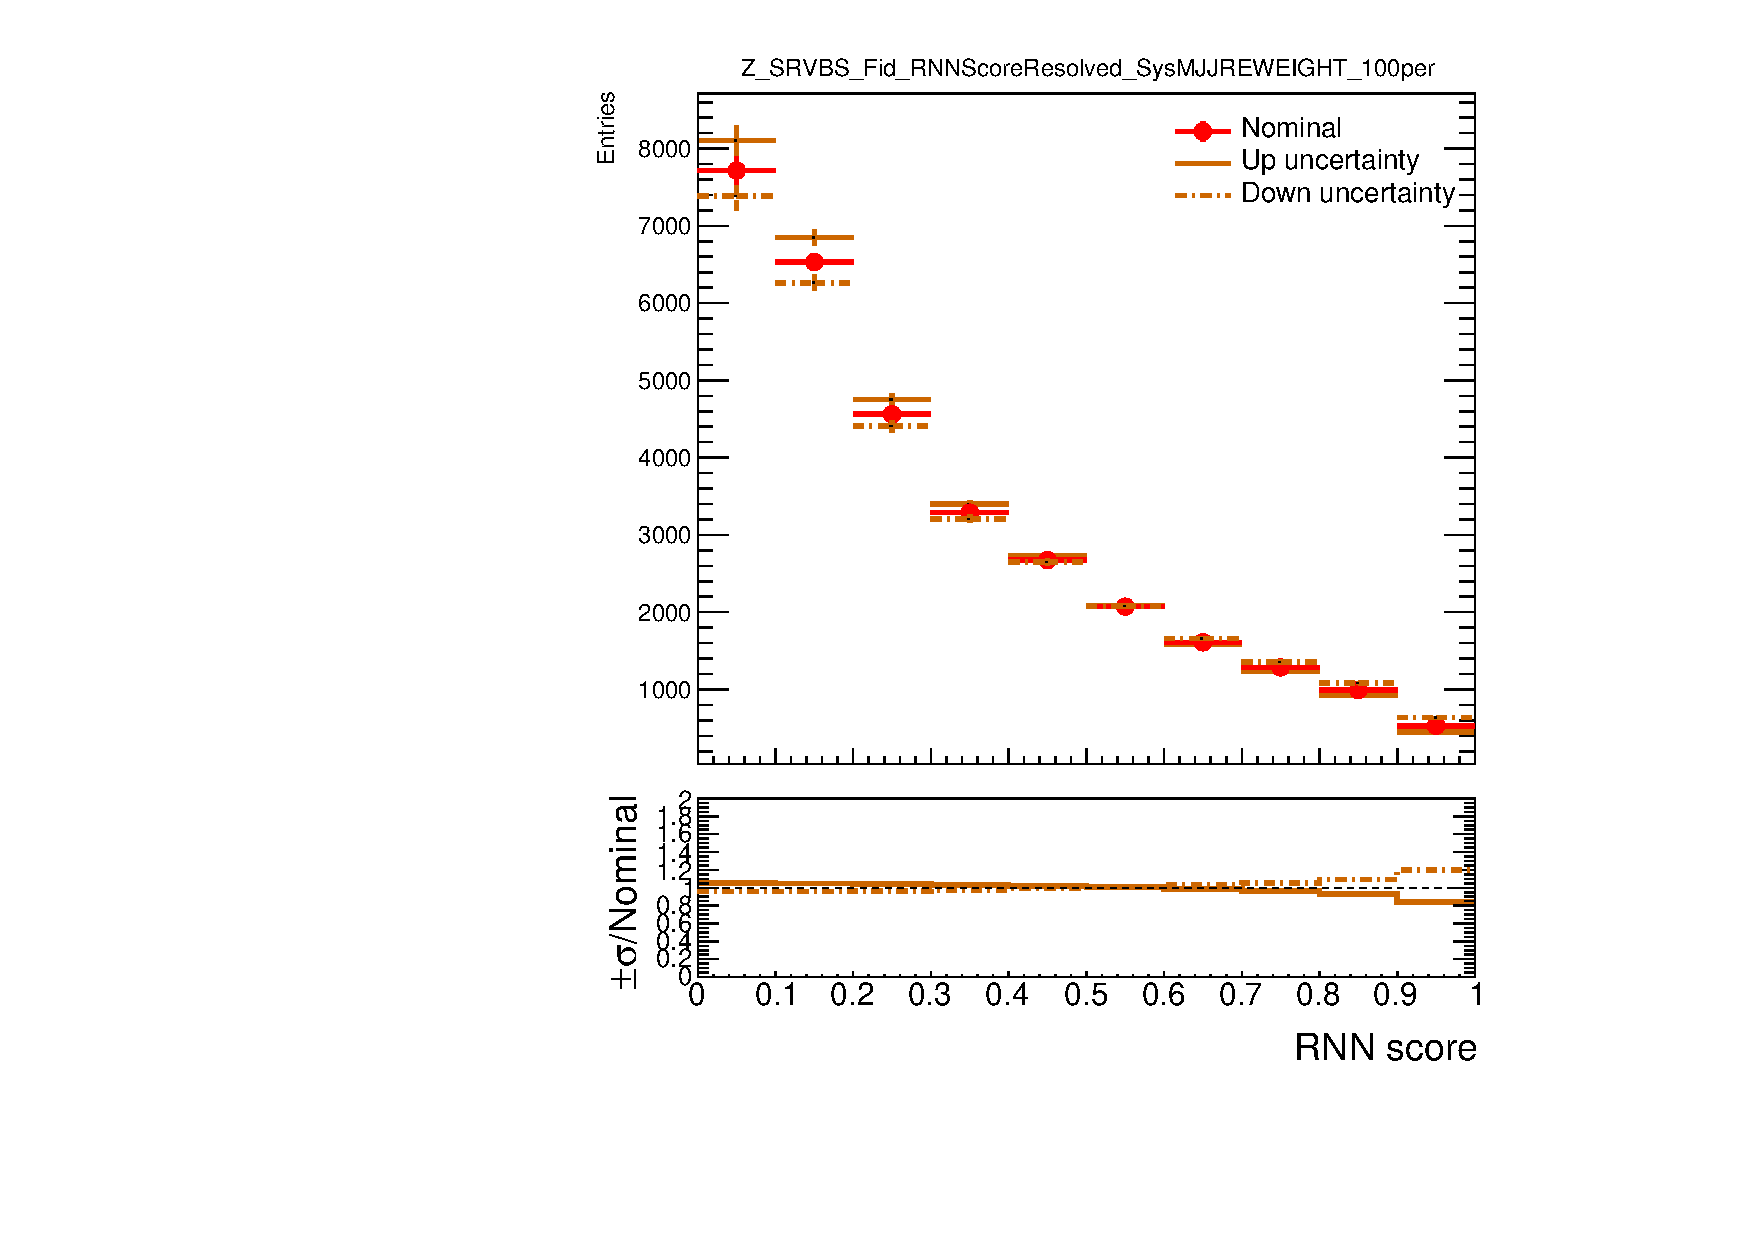
\includegraphics[width=0.32\textwidth,keepaspectratio]{figures/syst/Z_0ptag2pjet_0ptv_SRVBS_Fid_RNNScoreResolved_SysMJJREWEIGHT_100per.pdf}
 \caption[f]{
Pre-fit variation of the reweighting uncertainty of Z+jets sample in the 2-lepton channel.
}
\label{fig:mjjreweighting}
\end{center}
\end{figure}

\subsection{Generator difference uncertainites}
The difference of the distribution after the reweighting and the distribution using the alternative sample (MadGraph + Phythia~8) is assigned as a modeling uncertainty for V+jets background. There is a large difference in the modeling of the different generators, Sherpa and MadGraph, and we cannot know exactly which models the data correctly or not, hence the difference by using different generators is taken into account as an uncertainty. The MadGraph distribution used to evaluate this uncertainty is not reweighted since it is well matched to the data in the control region as figure~\ref{fig:SherpaMadGraph} shows.
For the $t\bar{t}$ and the QCD diboson sample, the difference of the nominal sample and the alternative sample is also assigned as the uncertainty.
The nominal and the alternative sample used for $t\bar{t}$ is Powheg + Phythia and Powheg + Herwig respectively.
For diboson sample, nominal sample is Sherpa~2.2.1 and the alternative is Powheg + Pythia.
The pre-fit variation of Z+jets samples in the 2-lepton channel is shown in figure~\ref{fig:modelingZ}.
\begin{figure}[H]
\begin{center}
 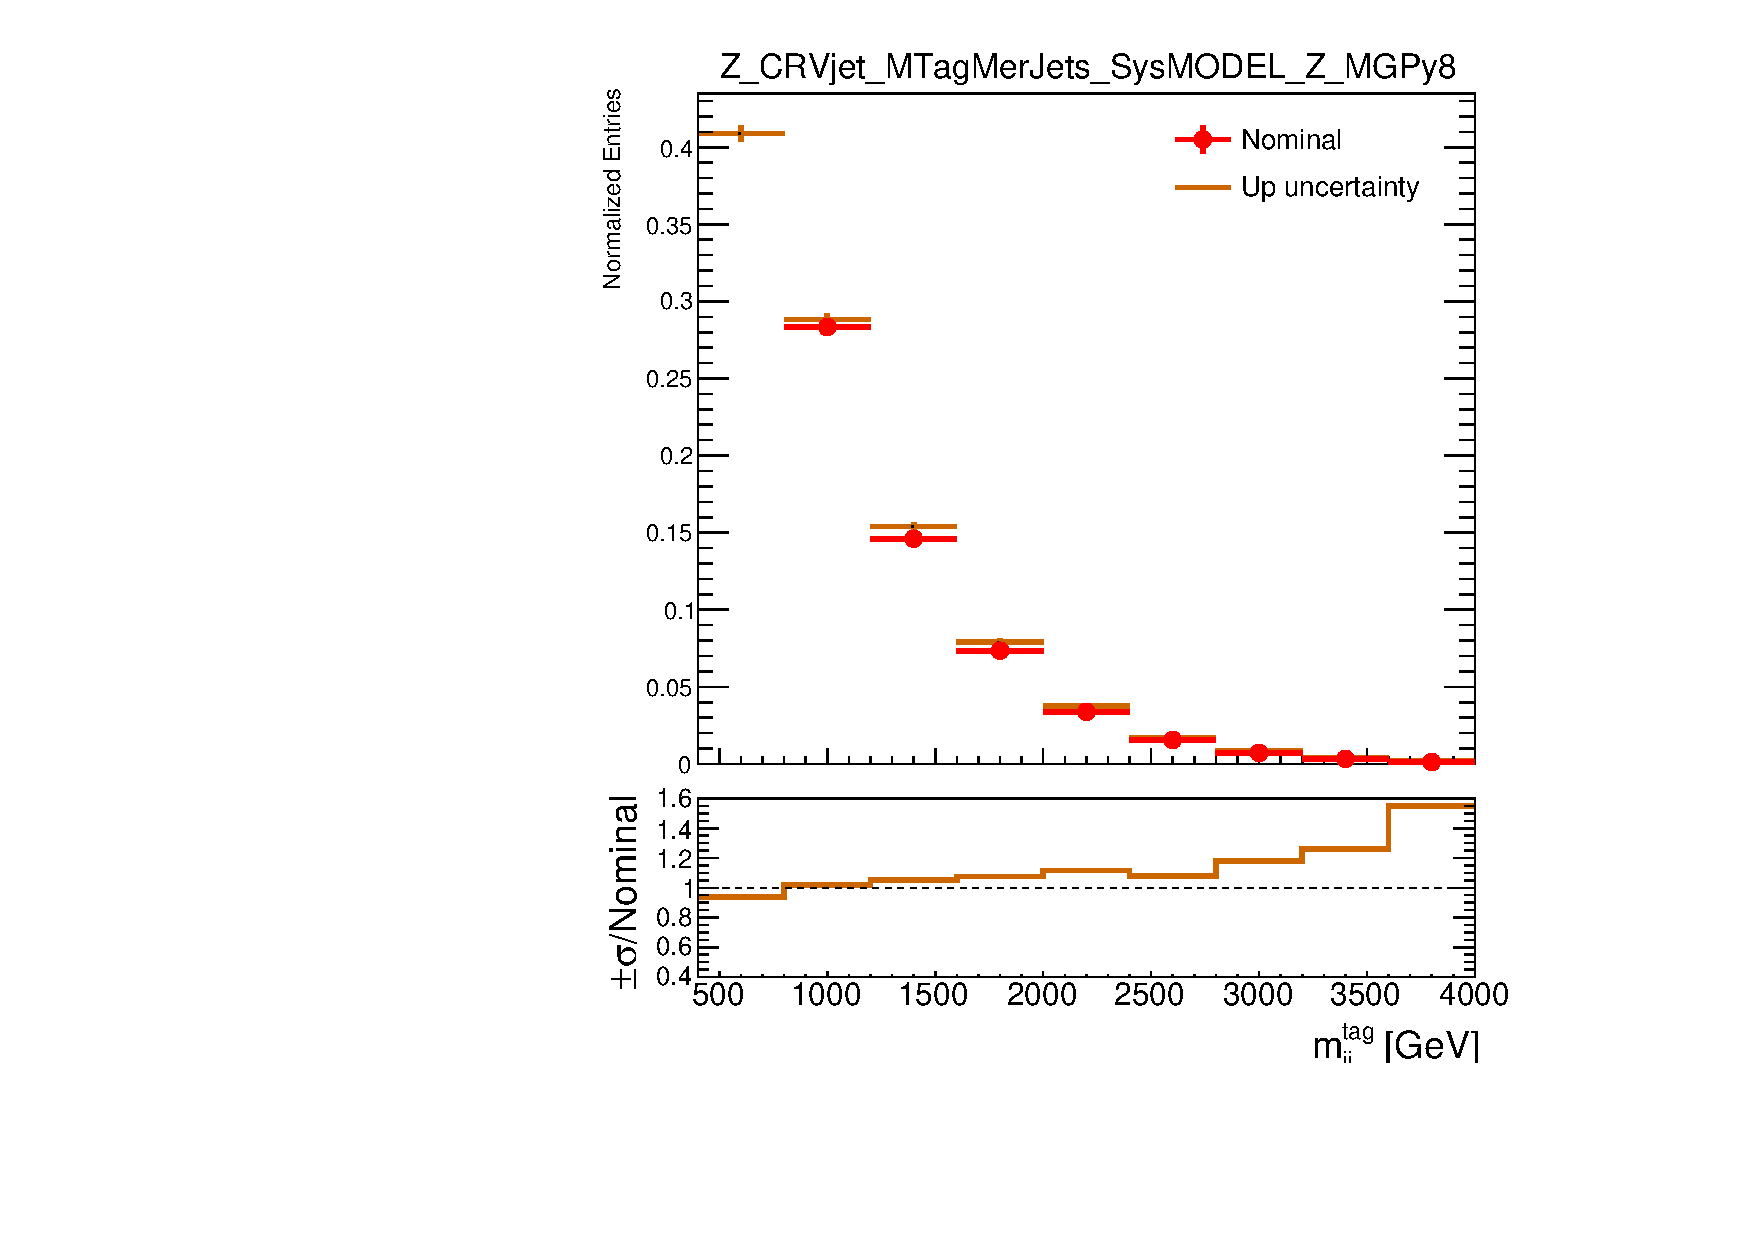
\includegraphics[width=0.32\textwidth,keepaspectratio]{figures/syst/Z_0ptag1pfat0pjet_0ptv_CRVjet_MTagMerJets_SysMODEL_Z_MGPy8_Norm.pdf}
 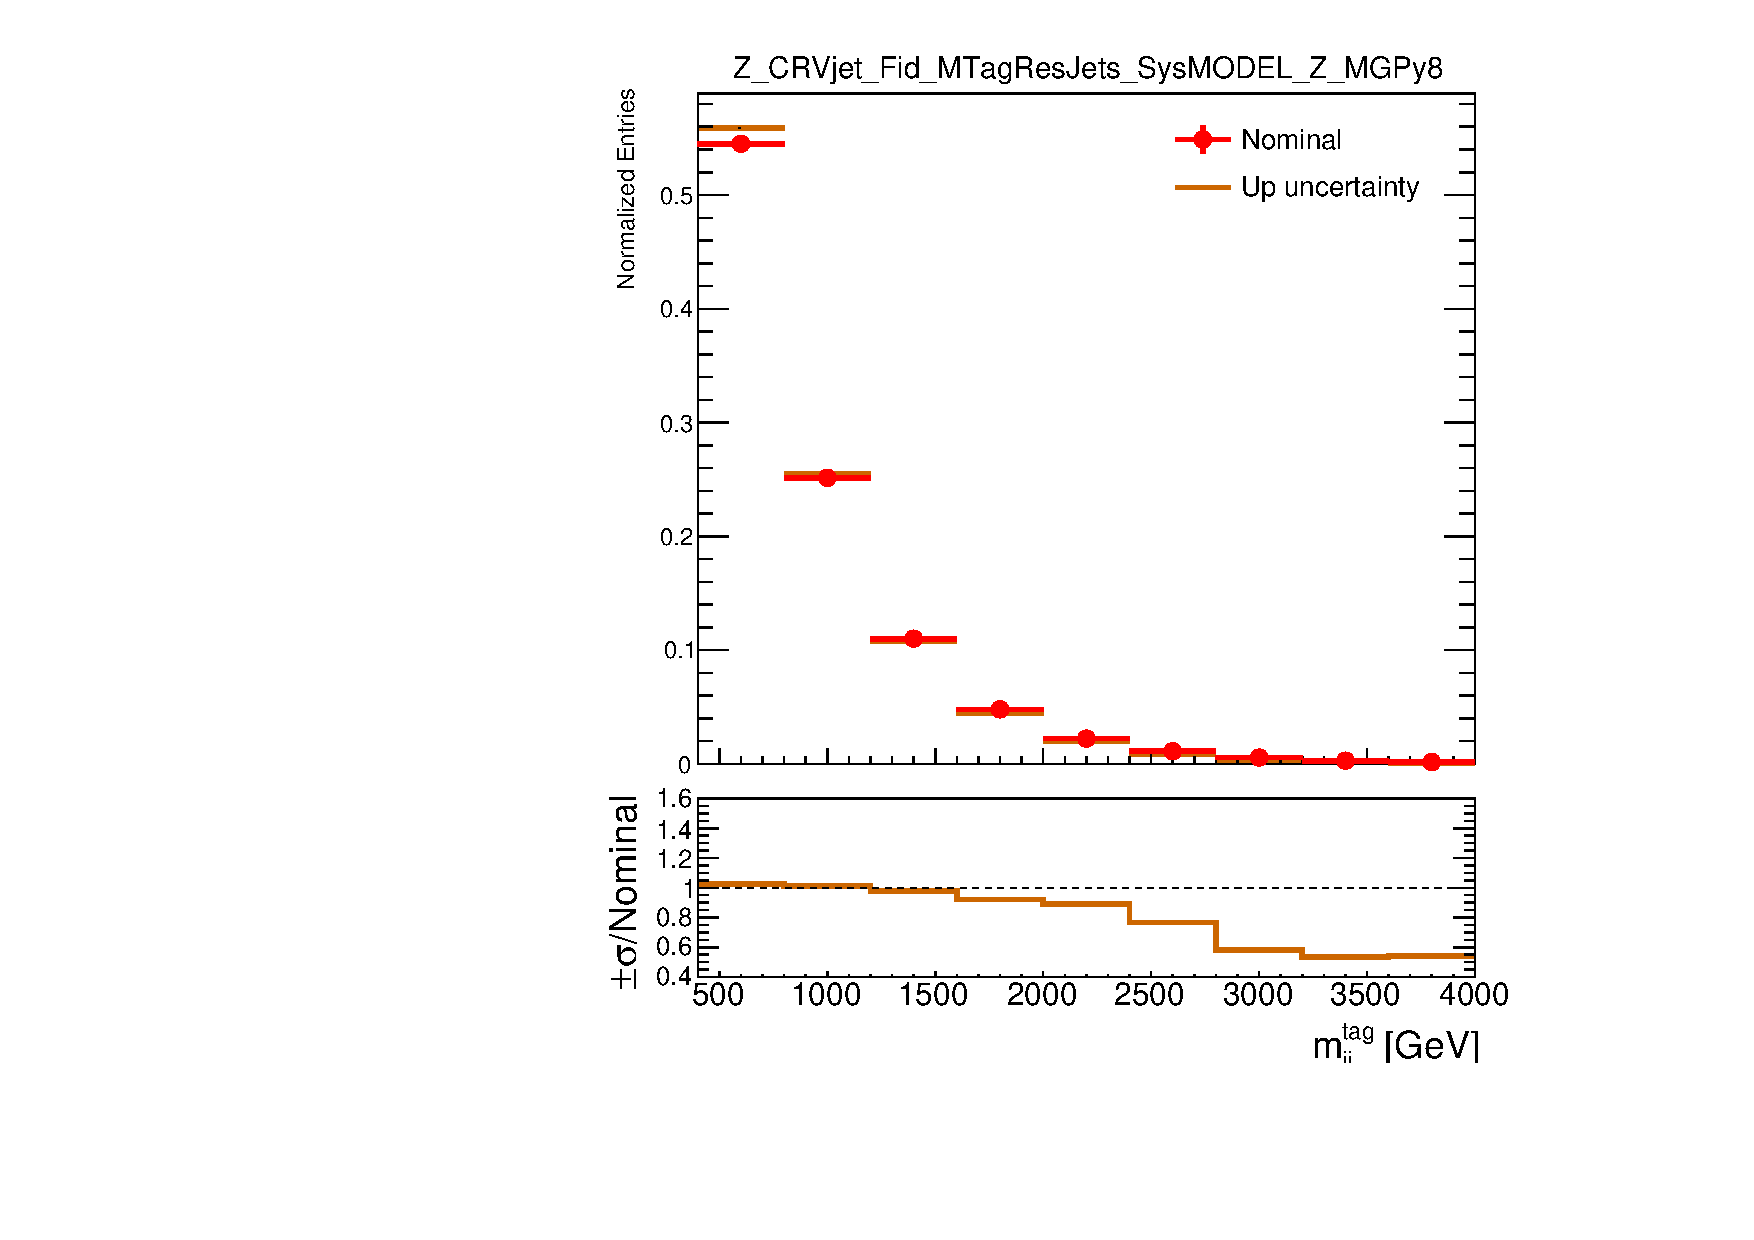
\includegraphics[width=0.32\textwidth,keepaspectratio]{figures/syst/Z_0ptag2pjet_0ptv_CRVjet_Fid_MTagResJets_SysMODEL_Z_MGPy8_Norm.pdf}
 \\
 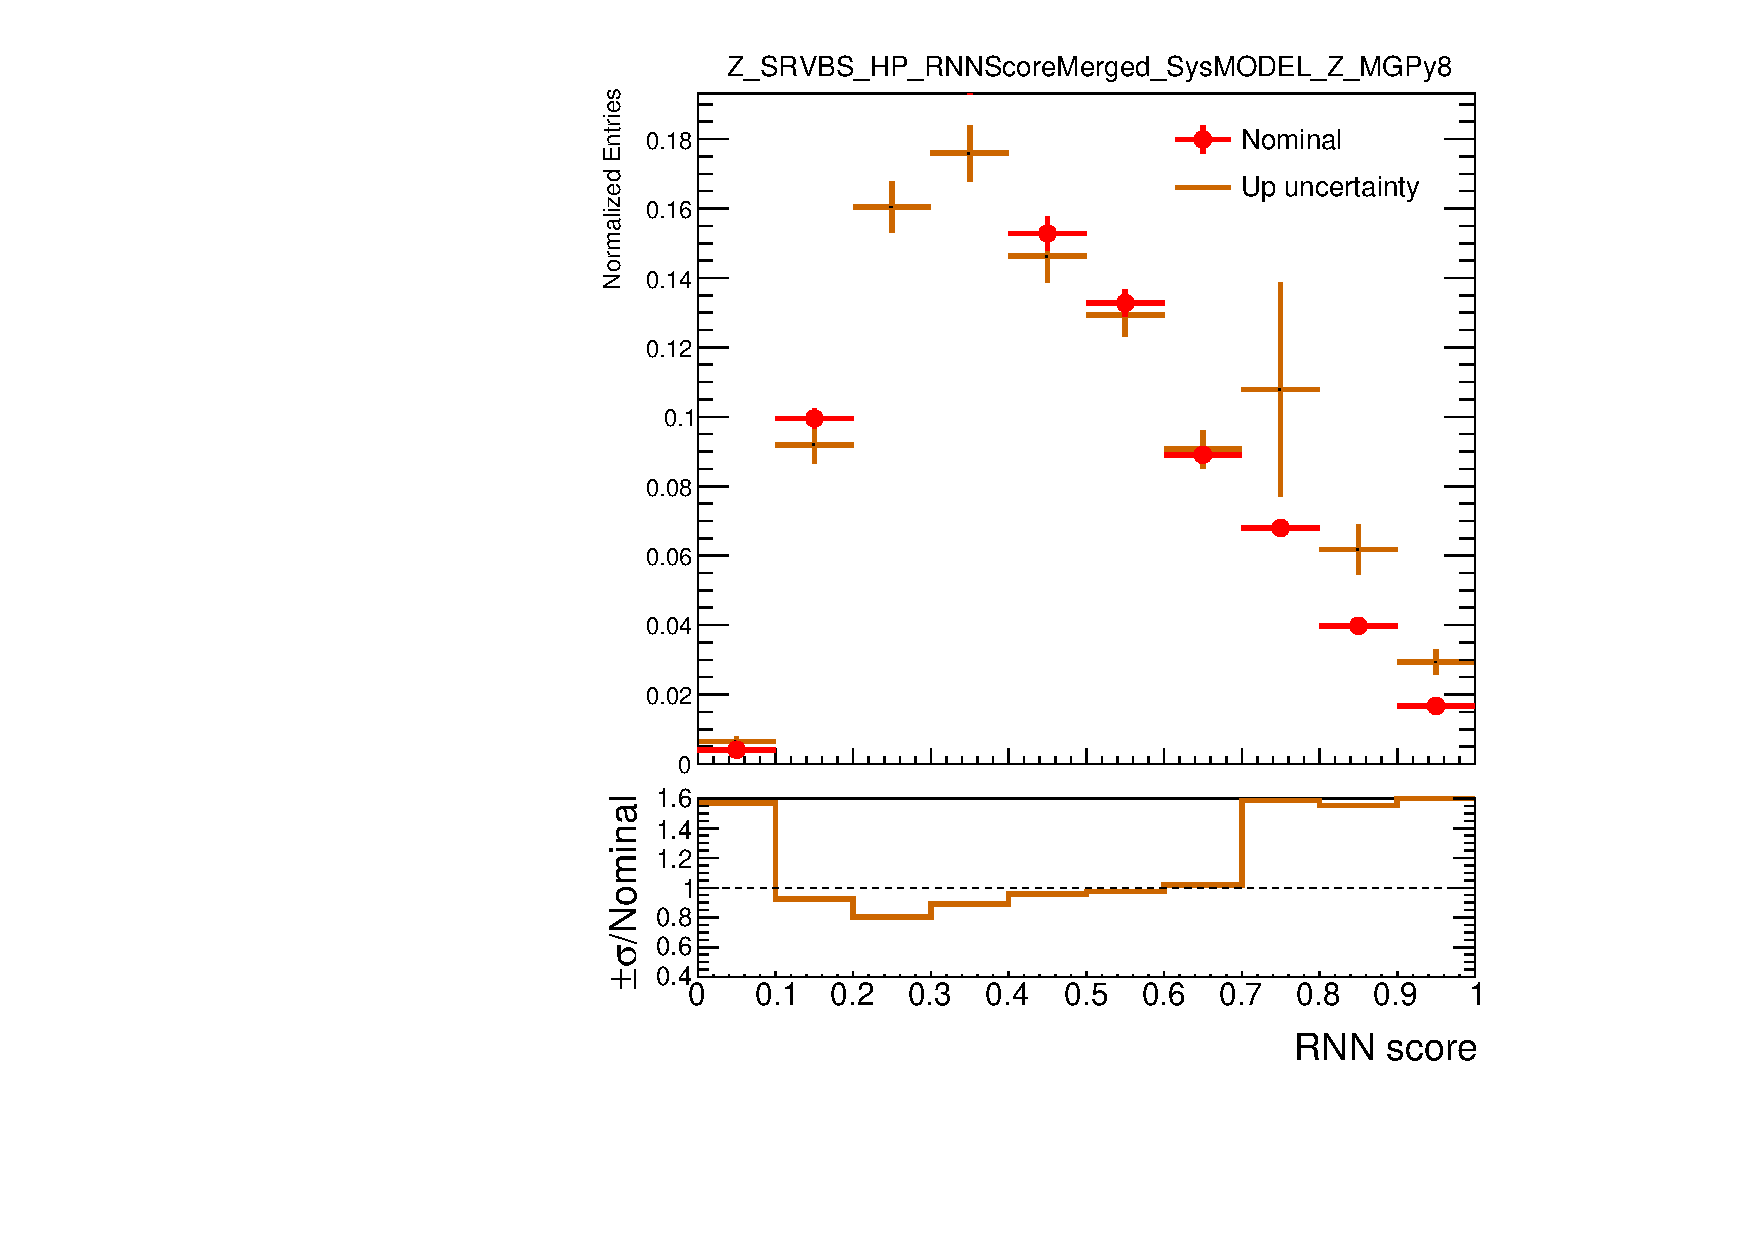
\includegraphics[width=0.32\textwidth,keepaspectratio]{figures/syst/Z_0ptag1pfat0pjet_0ptv_SRVBS_HP_RNNScoreMerged_SysMODEL_Z_MGPy8_Norm.pdf}
 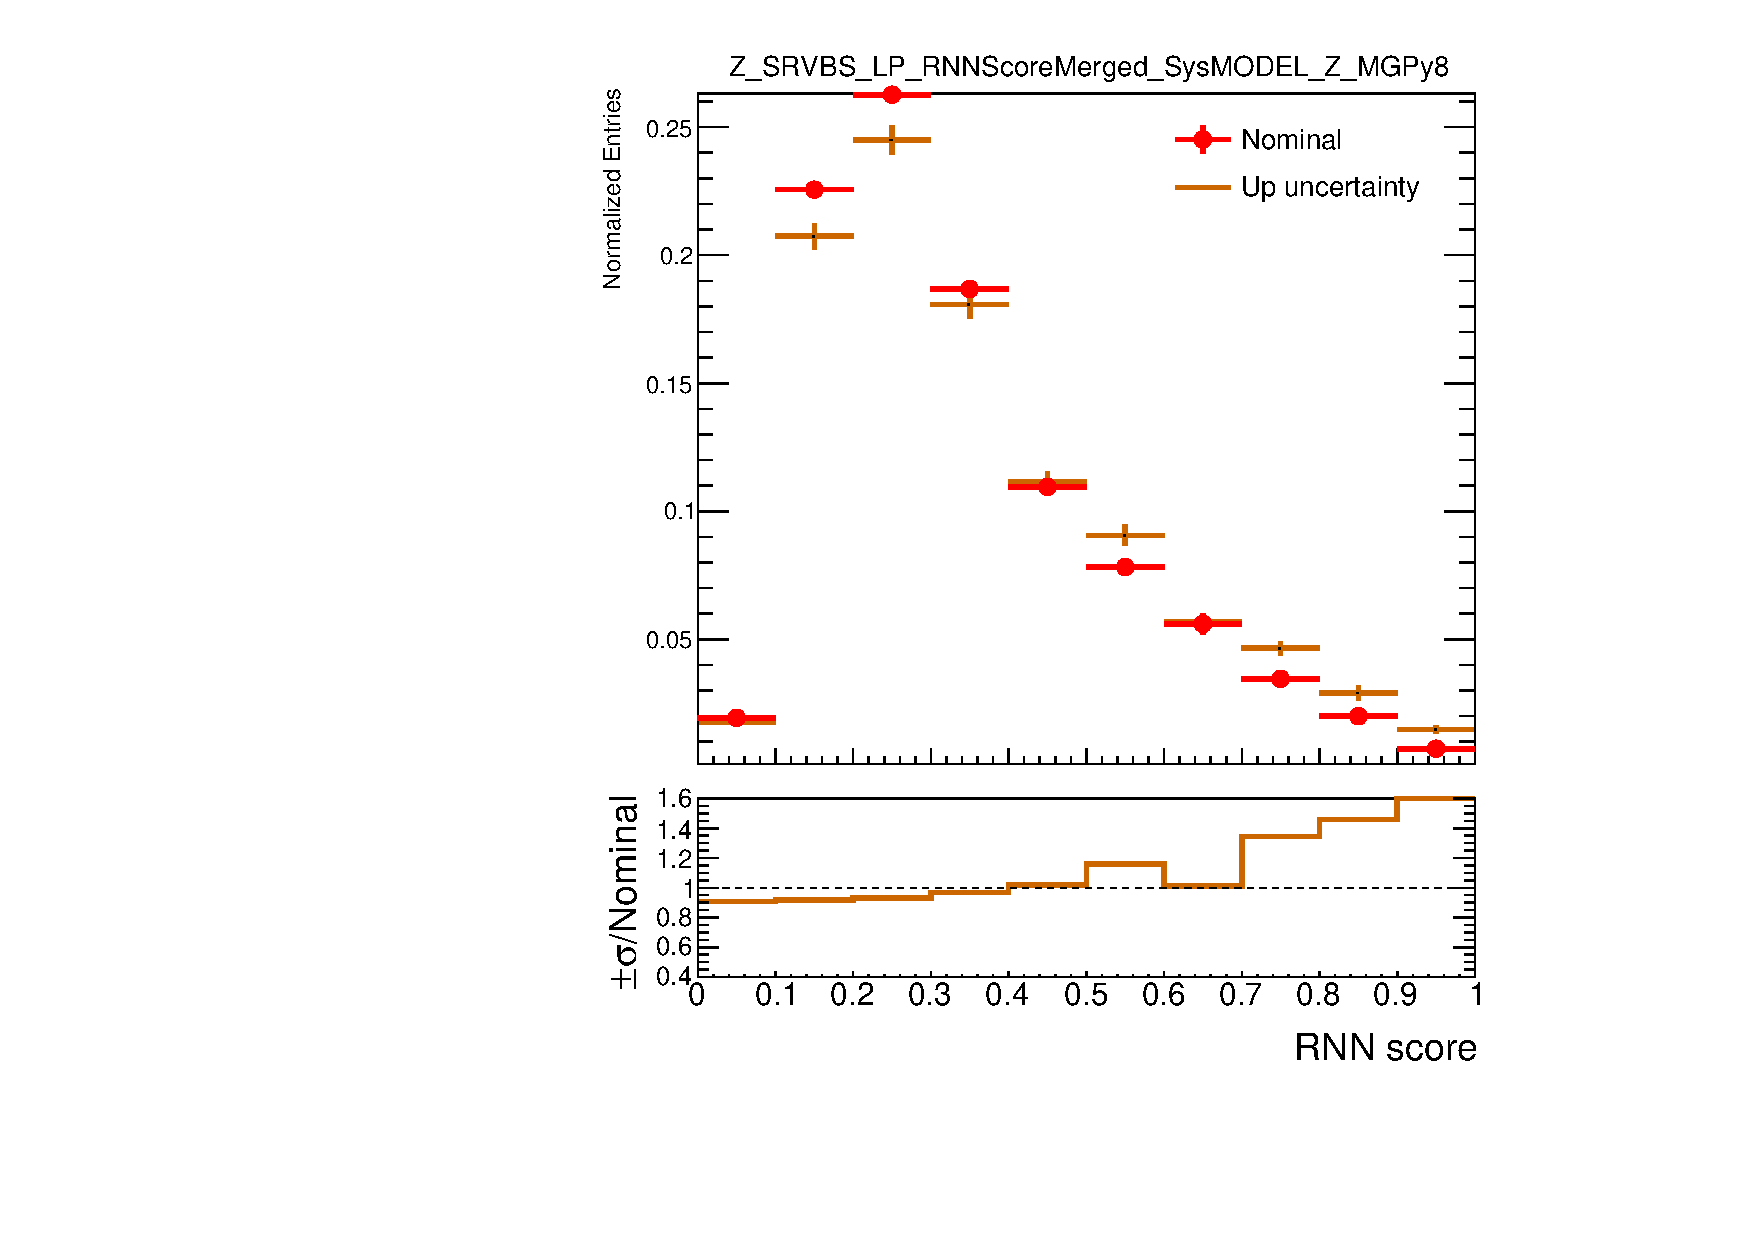
\includegraphics[width=0.32\textwidth,keepaspectratio]{figures/syst/Z_0ptag1pfat0pjet_0ptv_SRVBS_LP_RNNScoreMerged_SysMODEL_Z_MGPy8_Norm.pdf}
 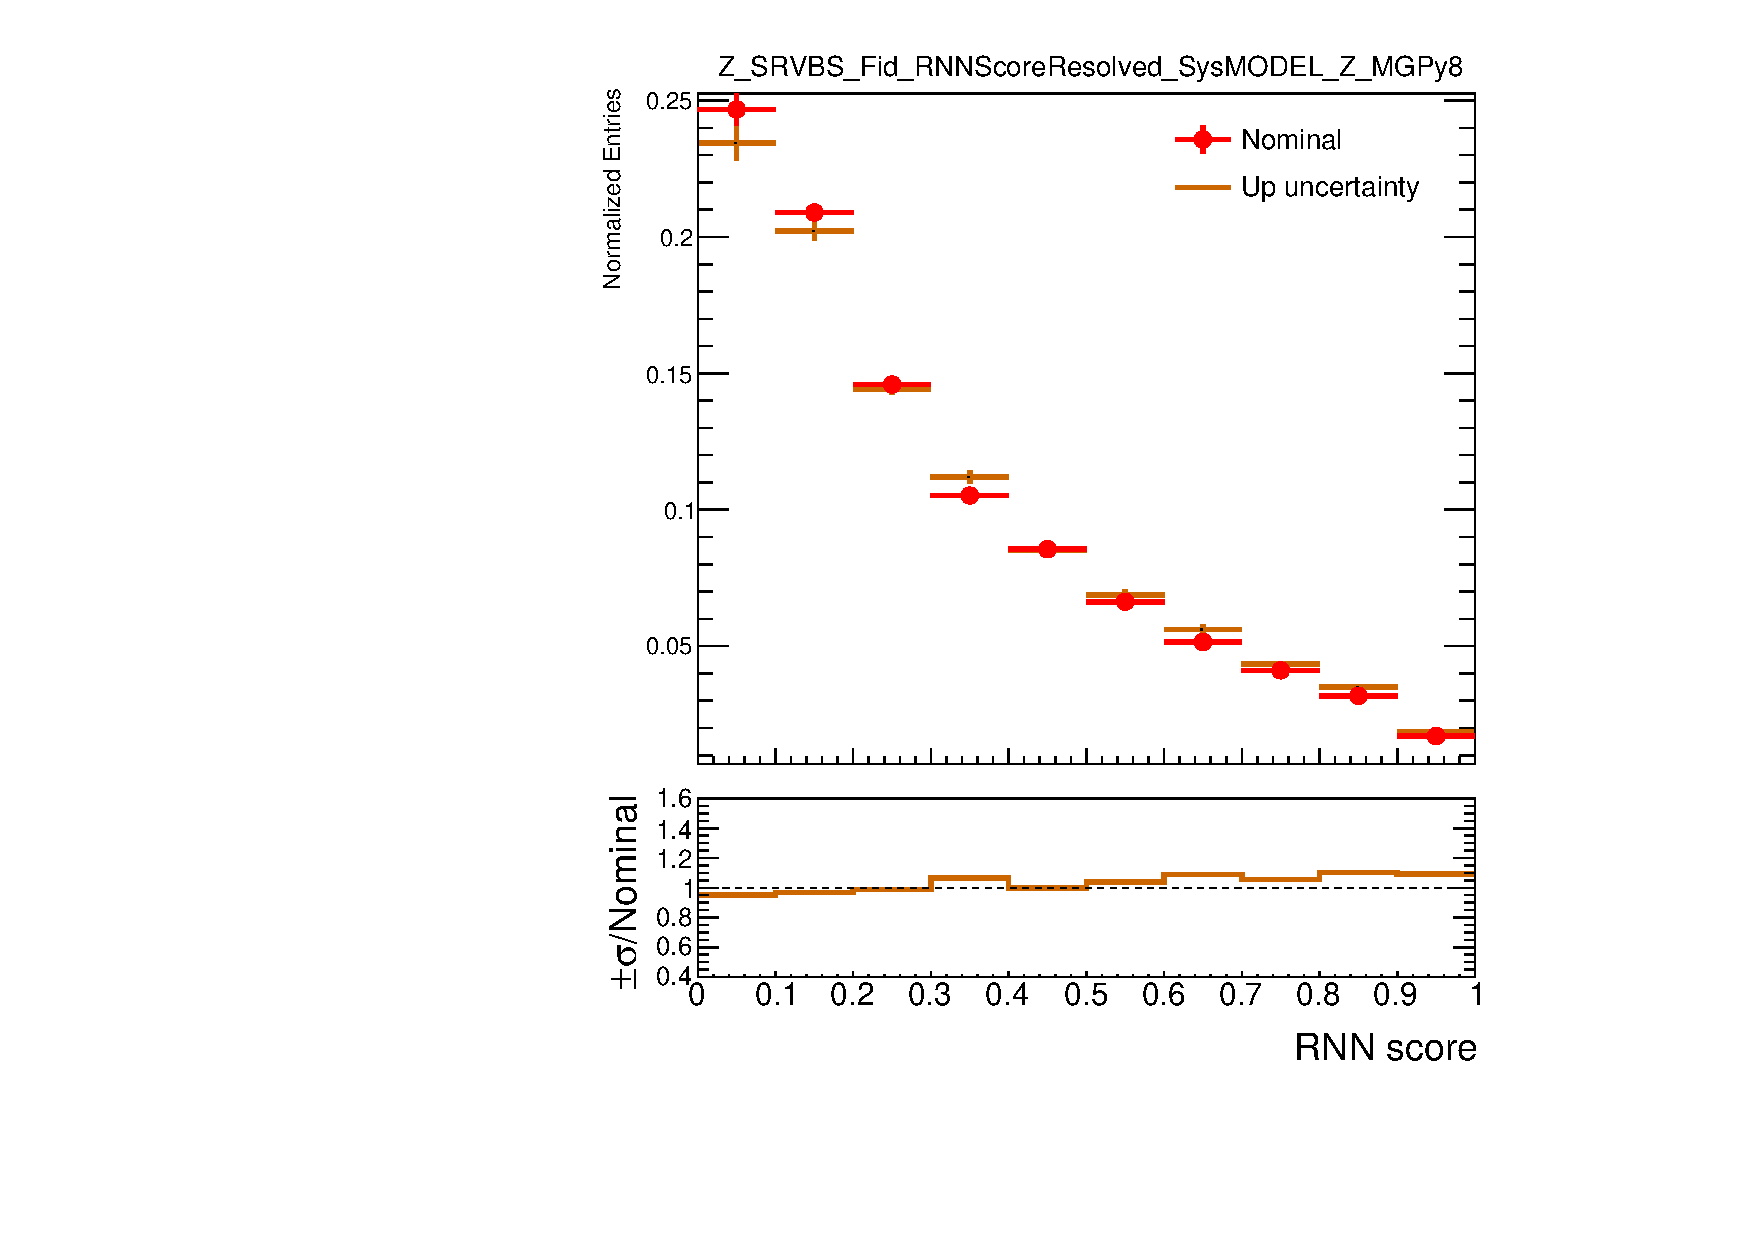
\includegraphics[width=0.32\textwidth,keepaspectratio]{figures/syst/Z_0ptag2pjet_0ptv_SRVBS_Fid_RNNScoreResolved_SysMODEL_Z_MGPy8_Norm.pdf}
 \caption[f]{
Pre-fit variation of the modeling uncertainty of Z+jets sample in the 2-lepton channel.  Variation distributions are normalized to the nominal one to see the shapes.
}
\label{fig:modelingZ}
\end{center}
\end{figure}

\subsection{QCD scale and PDF uncertainties}
\noindent\textbf{\sf{QCD scale uncertainties}}\\
QCD scale uncertainties are determined by varying the renormalization ($\mu_R$) and factorization ($\mu_F$) scale factor (\ref{subsec:factorization}) sets. 
%The renormalization scale $\mu_R$ is the scale at which the strong coupling $\alpha_s$ is evaluated, while the factorization scale $\mu_F$ is the scale to separate the perturbative part of the hard-interaction from the non-perturbative part of PDF as mentioned in section~\ref{subsec:factorization}. 
They are estimated by taking the envelope of the 6 set of the combination of the $\mu_R$ and $\mu_F$, which are fixed to be 1, 0.5, or 2.0. 
This uncertainties are implemented to the background samples as well as signal EW VV+jj sample.\\ \\
\noindent\textbf{\sf{PDF + $\alpha_s$ uncertainties}}\\
%
Parton Distribution Function (PDF) sets are obtained by the fit to experimental datasets. There are uncertainties originated from the experimental uncertainties from the datasets and from the choice of the functional form adapted in the PDF fits.
The uncertainty from the PDF set choice can be assessed by two approaches. One is to calculate the difference of a single PDF set by varying its internal parameters, which is called internal PDF uncertainties. For this study the 100 MC replicas of the NNPDF~\cite{Ball:2014uwa} sets are used. 
The standard deviation of the mean value of the 100 MC replicas for each bin of the final discriminant is taken as the uncertainty. 
%
An uncertainty on the strong coupling constant value, $\alpha_s$ is also considered. It is defined from the experimental uncertainties, and included to the estimation of the internal PDF uncertainties. 
The internal PDF uncertainty is considered both in V+jets background and the signal EW VV+jj samples.
%
The other is from the difference between the different PDF sets, which is called external PDF uncertainties. This uncertainty is estimated by comparing the nominal distributions with the alternative PDF sets. The uncertainties are combined by taking the envelope of all uncertainties, which means the most varied uncertainty is taken as the final uncertainty. 
External PDF uncertainty is considered only in V+jets background sample due to the missing of the alternative sample in signal.


%\section{Normalization}
%The list of the normalization of the backgrounds is shown in Table~\ref{tab:prior}.
%Some backgrounds are free floated, and others have gaussian priors. Since the Diboson background has a similar distribution with the electroweak signal (POI), it is difficult to constraints the normalization of the Diboson as a free floating parameter, therefore prior is set on it.
%\begin{center}
%\begin{tabular}{ |c|c|c|c|c| } 
%\hline
% & Background & float or with prior & prior \\
%\hline
%\multirow{3}{4em}{Merged} & Z & float &       \\ 
%& VV                          & prior &   0.5 \\ 
%& W                           & prior &   0.1 \\ 
%& ttbar                       & prior &   0.1 \\ 
%\hline
%\multirow{3}{4em}{Resolved} & Z & float &       \\ 
%& VV                          & prior &   0.3 \\ 
%& W                           & prior &   0.1 \\ 
%& ttbar                       & prior &   0.1 \\ 
%\hline
%\end{tabular}
%\caption{\label{tab:prior} The prior setting of the background normalization. }
%\end{center}

